\documentclass[compress]{beamer}
\usepackage[utf8]{inputenc}
\usepackage[francais]{babel}
\usepackage[T1]{fontenc}
\usepackage{amssymb}
\usepackage{amsmath}
\usepackage{amsfonts}
\usepackage{hyperref}
\usepackage[]{algorithm2e}
\usepackage{amssymb}
\usepackage{verbatim}
\usepackage{listings}
\usepackage{color}
\usepackage{graphicx}
\usepackage{subfig}
\usetheme[navigation]{UMONS}

\author{Benjamin André, Alexis Lecocq}
\title{Statistiques multidimensionnelles}
\subtitle[\ldots]{Réseaux de neurones (NN)}

\setbeamercovered{transparent} 
\setbeamertemplate{navigation symbols}{} 
\institute{UMONS\\Faculté des Sciences\\BA 3 Sciences Informatiques\\[2ex]
  
\includegraphics[height=4ex]{UMONS}\hspace{2em}%
  \raisebox{-1ex}{
\includegraphics[height=6ex]{UMONS_FS}}}
\date{Juin 2017} 
\definecolor{darkgreen}{rgb}{0.0, 0.2, 0.13}
\subject{Statistiques multidimensionnelles} 
\lstset{ %
  language=R,                     % the language of the code
  basicstyle=\footnotesize,       % the size of the fonts that are used for the code
  numbers=left,                   % where to put the line-numbers
  numberstyle=\tiny\color{gray},  % the style that is used for the line-numbers
  stepnumber=1,                   % the step between two line-numbers. If it's 1, each line
                                  % will be numbered
  numbersep=5pt,                  % how far the line-numbers are from the code
  backgroundcolor=\color{white},  % choose the background color. You must add \usepackage{color}
  showspaces=false,               % show spaces adding particular underscores
  showstringspaces=false,         % underline spaces within strings
  showtabs=false,                 % show tabs within strings adding particular underscores
  frame=single,                   % adds a frame around the code
  rulecolor=\color{black},        % if not set, the frame-color may be changed on line-breaks within not-black text (e.g. commens (green here))
  tabsize=2,                      % sets default tabsize to 2 spaces
  captionpos=b,                   % sets the caption-position to bottom
  breaklines=true,                % sets automatic line breaking
  breakatwhitespace=false,        % sets if automatic breaks should only happen at whitespace
  title=\lstname,                 % show the filename of files included with \lstinputlisting;
                                  % also try caption instead of title
  keywordstyle=\color{blue},      % keyword style
  commentstyle=\color{darkgreen},   % comment style
  stringstyle=\color{violet},      % string literal style
  escapeinside={\%*}{*)},         % if you want to add a comment within your code
  morekeywords={*,...}            % if you want to add more keywords to the set
} 

\begin{document}

	\begin{frame}
		\titlepage
	\end{frame}

	\begin{frame}
		\tableofcontents
	\end{frame}

	\section{Description de NN}
		\subsection{Machine Learning}
			\begin{frame}
				\frametitle{Machine Learning}
				Lorsque nous voulons résoudre un problème algorithmiquement, nous devons donner la marche à suivre exacte du programme qui mène à une solution.
				
				Dans certains cas, celle-ci est trop complexe que pour être écrite de cette façon, et les paramètres d'entrée (position, température, couleur,..) peuvent influencer le résultat de façon très complexe.
				
				L'approche du machine learning propose de trouver une solution approchée en minimisant l'erreur.
			\end{frame}
			
			\begin{frame}
				\frametitle{Machine Learning}
				\begin{alertblock}{Utilisation}
					Comme expliqué précédemment, il s'agit d'une solution approchée. Dans le cas ou il existe un algorithme efficace il sera préférable de l'utiliser.
				\end{alertblock}
				
				\begin{block}{Exemples}
					\begin{itemize}
						\item AlphaGo
						\item DeepBlue
						\item Voitures autonomes
						\item Filtre à spam
						\item Reconnaissance d'image
						\item Traduction
						\item Prévision de la bourse
					\end{itemize}
				\end{block}
			\end{frame}
		\subsection{Neural Networks (NN)}
			\begin{frame}
				\frametitle{Neural Networks}		
				\hspace{3em}%
				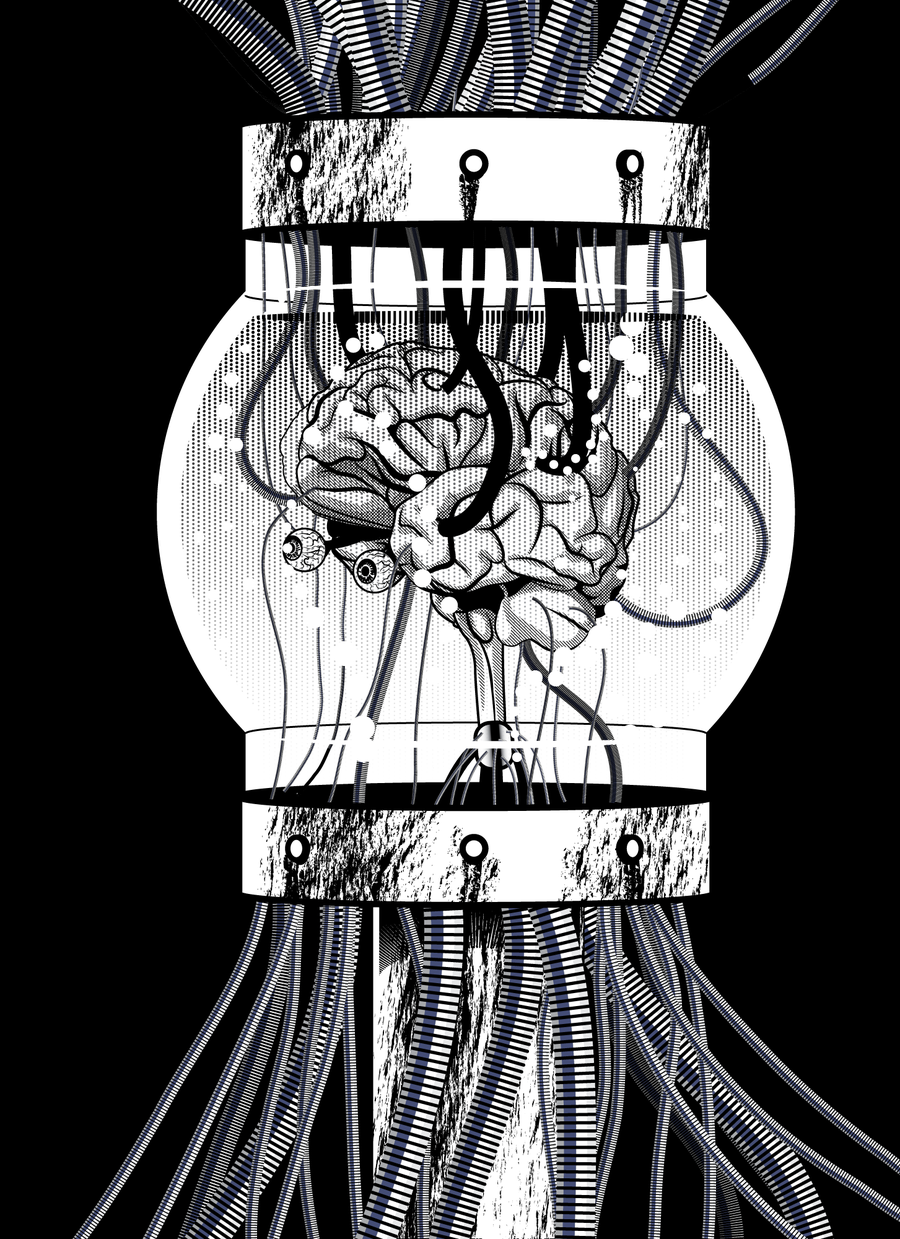
\includegraphics[height=100px]{img/brain}\hspace{2em}%
				\raisebox{-1ex}{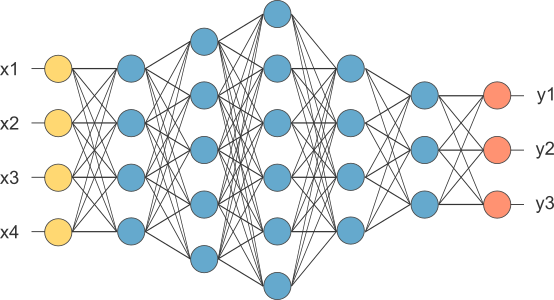
\includegraphics[height=100px]{img/deep_neural_network}}
				
				%Et ici on fait la blague qu'on pourrait penser au cerveau connecté et que ça fait peur, mais qu'en réalité... ça fait encore plus peur !
			\end{frame}


			\begin{frame}
				\frametitle{Neural Networks}
				\begin{block}{Types de réseaux de neurones}
					\begin{itemize}
						\item Deep Neural Network (DNN) : Réseau avec un grand nombre de couches.
						\item Convolutional Neural Network (CNN) : Inspiré du fonctionnement de la vue, les couches de neurones ici sont à plus d'une dimension.
						\item Recurrent Neural Network (RNN) : Réseau où la sortie est réintroduite dans le réseau pour les tests suivants : effet mémoire. 
					\end{itemize}
				\end{block}
				
				=> Nous nous concentrerons sur les DNN, avec peu de couche dans l'exemple (3).
			\end{frame}
	
			
			\begin{frame}
				\frametitle{Fonctionnement global}
					Dans le cas où on a $n$ paramètres, comment trouver $f(x_1, x_2, ..., x_n)$ ?
				
				
					Si la fonction est trop compliquée pour être écrite directement, on prend des \emph{exemples}, où l'on connaît déjà l'image par notre fonction pour certaines entrées. Typiquement, des milliers (millions). Ces exemples, nous les donnons à un réseau de neurones, constitué des fonctions mathématiques simples reliées par des arcs pondérés. Ils jouent le rôle \emph{d'axiome}.
					
					
					Nous donnons les exemples au réseau qui ajuste les poids pour approximer au mieux la fonction, tout en la généralisant.
					
					
					Maintenant, en lui présentant des variables, le réseau peut \emph{prédire} $f(x_1, x_2, ..., x_n)$.
			\end{frame}


		\subsection{DNN}
			\begin{frame}
				\frametitle{Structure des couches}
				3 types de couches :
				\begin{itemize}
					\item L'entrée : Couche correspondant aux variables à évaluer
					\item Les couches "cachée" : Couches correspondant au comportement interne du réseau, le nombre de couches dépend du problème, et il n'y a pas de règles prédisant le nombre de couches nécessaires. De nombreuses opérations mathématiques se font ici.
					\item La sortie : Couche retournant un nombre correspondant soit à une classe, soit à la valeur d'évaluation des paramètres d'entrées
				\end{itemize}
				
				Tous les neurones (décrits plus tard) sont dans une couche et une seule. Ceux-ci sont interconnectés avec tous les neurones de la couche précédente et tous ceux de la suivante, et rien d'autre (parfois avec un poids 0 cependant).
				
			\end{frame}


			\begin{frame}
				\frametitle{Couche cachée}
				\hspace{6em}%
				\vspace{6em}
				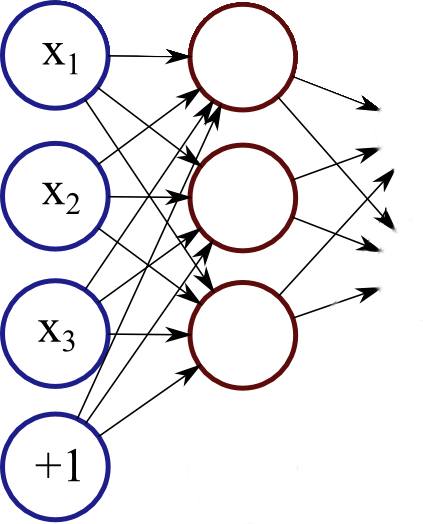
\includegraphics[height=120px]{img/hidden_layer}\hspace{2em}%
				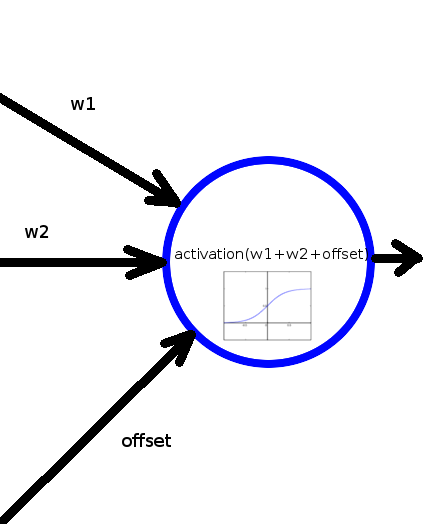
\includegraphics[height=120px]{img/neurone}
				\vspace{-4em}				
			\end{frame}
			
			\begin{frame}
				\frametitle{Fonction d'activation}
				Chaque neurone reçoit les valeurs de la couche précédente, ainsi qu'un offset, qui est propre à toute la couche actuelle.
				Il en effectue une transformation linéaire (ici, avec les poids 1, 1, 1), mais on pourrait très bien imaginer $activation(0.2*w1 + 1.4*w2 - 2.1)$.
				Le soucis, c'est qu'on pourrait vite finir avec des résultats très grand, si notre fonction d'activation ne présente pas de caractéristique spécifique : être bornée sur le domaine des images (et continue).
				
				La fonction d'activation appliquée sur la transformation linéaire la plus répandue est la sigmoïde, qui retourne un résultat entre 0 et 1 : 
				$$  \frac{1}{1 + e^{-x}} $$				
			\end{frame}

			
			\begin{frame}
				\frametitle{Backpropagation}
				\begin{alertblock}{C'est fini ?}
					On a un réseau de neurones, c'est bien beau, mais comment définir les poids ?
				\end{alertblock}
				
				Il existe plusieurs stratégies pour les initialiser, mais il est tout à fait valable de commencer avec des poids aléatoires.
				Vous vous souvenez des exemples pour l'entraîner ? C'est ici qu'ils interviennent ! On nourrit le réseau avec les exemples un à un. On compare sa réponse avec le résultat attendu. Le taux d'erreur est très élevé au début.
				
				Heureusement ! Il existe un algorithme pour ajuster les poids \emph{en détectant lequel est le plus responsable de l'erreur}. Il s'agit de la backpropagation !				
			\end{frame}


			%Mettre un beau schema de la BP, avec les delta
			% L'expliquer
			
			
			%Attaquer l'exemple
				%Choix du jour : DNN, exemple via les données de Boston (prix de l'habitation), avec un module neuralnet de R
				%Utilisation du set de Boston
				%Vérification : est-ce qu'il manque des valeurs ?
				%Separation des donee de train et de test
				%Normalisation de la matrice vers [0,1]
				%Entrainement
				%Test sur les données restantes
				%Comparaison du resultat du NN avec la realite
				%Test sur 10 exemples (melange des donnes)
				%Pour generer une probabilite sur l'erreur de notre reseau
				%Boite a moustache

\section*{Sources}
\begin{frame}
\frametitle{Sources}
	\url{https://www.r-bloggers.com/fitting-a-neural-network-in-r-neuralnet-package/}\\
	\url{http://www.parallelr.com/r-deep-neural-network-from-scratch/}\\
	\url{https://www.youtube.com/watch?v=BR9h47Jtqyw}\\
	\url{http://doctor-morbius.deviantart.com/}\\
	\url{https://datascienceplus.com/fitting-neural-network-in-r/}%d'ou on tient le code !
\end{frame}

\end{document}